\chapter{Dealing with File Bloat}\label{ch:bloat}
\redmarginpar{Have done the groundwork for this chapter (results in table~\ref{tab:filesize}) but need to do some more on comparing different compression schemes, and then write about it.}

\section{Rationale}
In the system thus far described in this thesis, the emphasis has been firmly upon reducing the computational complexity of layout operations at view-time of a document, and therefore little consideration has been given to the filesize of the resultant malleable documents.

\todo{Put in some pdfdump output comparing ``normal'' pdfs with my malleable ones (maybe as an appendix)}

The resultant tradeoff between filesize and required computation has previously been justified on the basis that storage is both cheap (as of 2013 one US dollar will buy around two gigabytes of \textsc{nand} flash memory) and light; and batteries, although not enormously expensive either, already comprise a significant proportion of the overall mass of most portable devices suitable for reading \ebook{}s. The upshot is that adding more storage to a device has little impact upon devices' aesthetics, but that adding extra battery life (emerging nanotube battery technology notwithstanding) would result in vast increases in the devices' overall bulk and mass.

Despite this, it seems perverse to make no attempt at all to keep filesizes as small as possible, as long as there are no (or limited) impacts upon the required computation at view-time.

\section{Implementation}
The most obvious saving that can be made is with the duplication of a document's textual content. The systems described in chapters \ref{ch:malleable}~and~\ref{ch:floats} both contain as many copies of the document text as there are pre-rendered galleys; in practice, though, there is no real need for more than one copy to be present in the file. Two approaches to this problem were considered.

\subsection{Pointers into the Source Text}
The first approach to be considered was to include the source text of the document in its entirety, and for each rendering to contain only pointers to the relevant sections of text, instead of the words themselves. These pointers can either be physical\redmarginpar{I don't think ``physical'' is the right word here. What is???} (in the form of a character offset from the start of the text) or logical (in the form \emph{paragraph m, word n}). If the document text is to be included as a plaintext string, physical pointers are easier to use than logical: logical pointers either require an auxiliary data structure to map the logical pointers to physical ones, or for the document text to be stored in a format reflecting the logical structure, \ie{} not in plain text.

A drawback of using this approach is that on occasion, the output of the linebreaking process does not exactly match the input: for example in the case where words are hyphenated (requiring one word to be broken into two parts, and the addition of a hyphen) or where certain glyphs may be substituted for others (such as with the use of ligatures, where a glyph pair or triplet may be replaced with a single glyph).



\subsection{Use of a Dictionary}
The second approach considered was the use of a \emph{dictionary} (or \emph{map}) to act as a lookup table for each word-level item produced by the linebreaking process.

\begin{figure}
  \begin{center}
  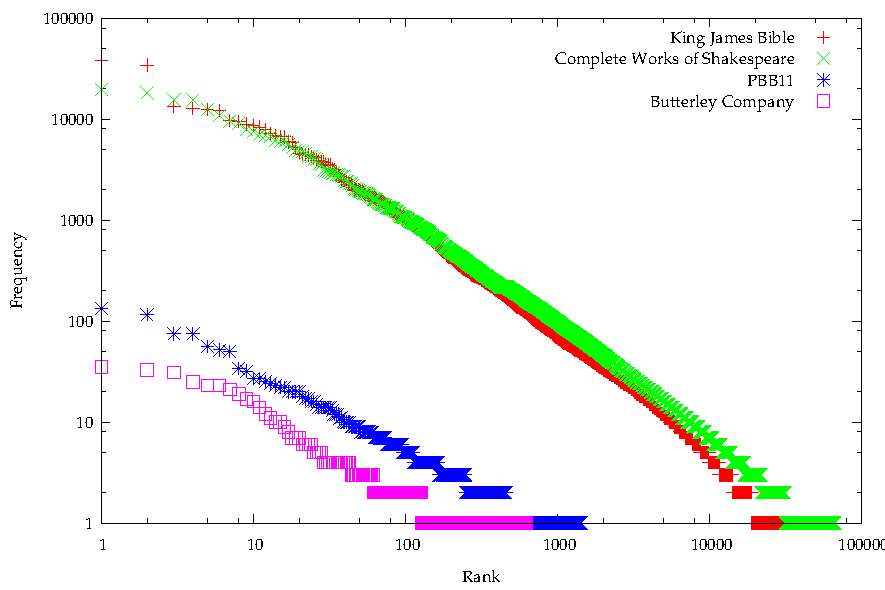
\includegraphics[width=\textwidth]{gfx/wordfreq}
  \end{center}
  \caption[Word frequencies in various documents]{Word frequencies in various documents, plotted on a log-log scale. All of these documents, despite their varying lengths, appear to conform well with Zipf's Law. }
  \label{fig:wordfreq}
\end{figure}

If, for example, if the word ``shall'' appears several times in a document (in the King James Version of the Bible it appears 9760 times, and in the complete works of Shakespeare 3016 times) it is only stored once in the dictionary. As long as a word's key is lexicographically shorter than the word itself, it can be guaranteed that some redundancy has been removed from the data.


\section{Results}

\subsection{Ordered dictionary with absolute positioning}

\begin{figure}
  \begin{center}
  \includegraphics[width=\textwidth]{gfx/scaling}
  \end{center}
  \caption[Filesize versus number of renderings, using absolute positioning]{Filesize in bytes, for a selection of documents that contain varying numbers of galley renderings, using an ordered dictionary and absolute positioning}
  \label{fig:sizescale}
\end{figure}

\begin{figure}
  \begin{center}
  \includegraphics[width=\textwidth]{gfx/scalingpersrc}
  \end{center}
  \caption[Filesize as a proportion of source document size, versus number of renderings, using absolute positioning]{Filesize as a proportion of source document filesize, for a selection of documents that contain varying numbers of galley renderings, using an ordered dictionary and absolute positioning}
  \label{fig:sizescalepersrc}
\end{figure}

\begin{figure}
  \begin{center}
  \includegraphics[width=\textwidth]{gfx/scalingpersrcpern}
  \end{center}
  \caption[Filesize as a proportion of source document size, per rendering, versus number of renderings, using absolute positioning]{Filesize as a proportion of source document filesize and per galley rendering, for a selection of documents that contain varying numbers of galley renderings, using an ordered dictionary and absolute positioning}
  \label{fig:sizescalepersrcpern}
\end{figure}


\subsection{Ordered dictionary with relative positioning}

\begin{figure}
  \begin{center}
  \includegraphics[width=\textwidth]{gfx/scalingdeltas}
  \end{center}
  \caption[Filesize versus number of renderings, using relative positioning]{Filesize in bytes, for a selection of documents that contain varying numbers of galley renderings, using an ordered dictionary and relative positioning, with word widths stored in the dictionary}
  \label{fig:sizescaledeltas}
\end{figure}

\begin{figure}
  \begin{center}
  \includegraphics[width=\textwidth]{gfx/scalingdeltaspersrc}
  \end{center}
  \caption[Filesize as a proportion of source document size, versus number of renderings, using relative positioning]{Filesize as a proportion of source document filesize, for a selection of documents that contain varying numbers of galley renderings, using an ordered dictionary and relative positioning, with word widths stored in the dictionary}
  \label{fig:sizescaledeltaspersrc}
\end{figure}

\begin{figure}
  \begin{center}
  \includegraphics[width=\textwidth]{gfx/scalingdeltaspersrcpern}
  \end{center}
  \caption[Filesize as a proportion of source document size, per rendering, versus number of renderings, using relative positioning]{Filesize as a proportion of source document filesize and per galley rendering, for a selection of documents that contain varying numbers of galley renderings, using an ordered dictionary and relative positioning, with word widths stored in the dictionary}
  \label{fig:sizescaledeltaspersrcpern}
\end{figure}

\begin{table}
    \myfloatalign
  \begin{tabularx}{\textwidth}{lXXXXXX} %\toprule
    & \multicolumn{2}{l}{\textsc{source text}} & \multicolumn{2}{l}{\textsc{orig. scheme}} & \multicolumn{2}{l}{\textsc{dictionary}} \\
    & \textsc{plain} & \textsc{gz} & \textsc{plain} & \textsc{gz} & \textsc{plain} & \textsc{gz} \\ \midrule
    PBB11~\cite{Pinkney2011} & 23\textsc{k} & 9.4\textsc{k} & 627\textsc{k} & 145\textsc{k} & 314\textsc{k} & 111\textsc{k} \\ \midrule
    King James Bible & 4.3\textsc{m} & 1.4\textsc{m} & 144\textsc{m} & 32\textsc{m} & 73\textsc{m} & 24\textsc{m} \\ 
    \bottomrule
  \end{tabularx}
  \caption[Comparison of filesizes]{Comparison of filesizes using various encoding methods}  \label{tab:filesize}
\end{table}